% !TEX root = ./../../main.tex
\subsection{Using the Least Squares Method for Finding Parameters of Best Fit Curves}
\label{sec:least squares}

\subsubsection{Finding Best Fit Parameters}

For the next part, we will use the method of least squares to find fit parameters of a function from some data. 
We are given some independent measurements (see \autoref{tab:appendix:least_squares_data}).
Assuming the data came from a third-order polynomial, the fit function is of the form:
\begin{gather}
    \label{eq:least_squares:fit_polynomial}
    y(x) = θ_0 + θ_1 x + θ_2 x^2 + θ_3 x^3.
\end{gather}
This kind of polynomial function is linear in its parameters (the coefficients \( θ_i \)), meaning an exact solution exists. For a set of \( n \) inputs $\vec{x}$, our model predicts outputs: $ \vec{\mu} = \mat{A} \vec{\theta} $, with $ A_{ij} = x_i^j$. When given measurement data, $\vec{x}$ represents the independent variable and $\vec{y}$ represents the dependent variable.
This lets the sum of the square residuals ($\chi^2$) be calculated:
\begin{equation}
    \label{eq:least_squares:sum_square_residuals_matrix_representation}
    \chi^2 = (\vec{y} - \mat{A}\vec{\theta})\transpose \mat{C}^{-1} (\vec{y} - \mat{A}\vec{\theta}).
\end{equation}
$\mat{C}$ is the matrix representing the covariances of $\vec{y}$.
After taking the gradient of this expression and setting to zero, matrix algebra finds us the estimate $\hat{\vec{\theta}}$ which minimizes the square residuals.
\begin{equation}
    \label{eq:least_squares:finding_theta}
    \hat{\vec{\theta}} = (\mat{A}\transpose \mat{C}^{-1} \mat{A})^{-1} \mat{A}\transpose \mat{C}^{-1} \vec{y} \eqcolon \mat{G} \vec{y}
\end{equation}
To find the covariances $\mat{C}_{\vec{\theta}} $ of our fit parameters, we transform \( \mat{C} \):
\begin{equation}
    \label{eq:least_squares:covariances_theta}
    \mat{C}_{\vec{\theta}} = \mat{G} \mat{C} \mat{G}\transpose  = (\mat{A}\transpose \mat{C}^{-1} \mat{A})^{-1}.
\end{equation}

Translating these matrix operations into code gives an analytic solution for the least squares regression.
For the given data, we find the following fit parameters and covariances:
\begin{gather}
    θ_0 = \num{ 4.4 \pm 0.3}, \quad
    θ_1 = \num{-0.4 \pm 0.8}, \quad
    θ_2 = \num{-2.6 \pm 0.4}, \quad
    θ_3 = \num{ 2.3 \pm 0.5}, \\
    \mat{C}_{\vec{θ}} = 
    \begin{pmatrix}
        \num{ 0.114 } & \num{-0.0261} & \num{-0.0879} & \num{ 0.0163} \\
        \num{-0.0261} & \num{ 0.566 } & \num{ 0.0111} & \num{-0.334 } \\
        \num{-0.0879} & \num{ 0.0111} & \num{ 0.170 } & \num{-0.0172} \\
        \num{ 0.0163} & \num{-0.334 } & \num{-0.0172} & \num{ 0.257 }
    \end{pmatrix}.
\end{gather}

\subsubsection{Numerical Minimization for Finding Best Fit Parameters}

In this problem, it was relatively easy to outline an analytic solution which minimizes the square residuals and produces an optimized fit. However, this approach does not work in general, especially with more complicated functions. For some, there might not even be an analytic solution. Because of this, it is important to note that we can alternatively use numerical tools to find the fit parameters which minimize \( \chi^2 \).

To find a fit curve, we also used the \verb|iminuit| python package.
Specifically the \verb|Minuit|, \verb|.migrad()| and \verb|.minos()| tools helped us find the best values for all the \( \theta_i \). 
The results match quite well, which can be seen visually in \autoref{fig:least_squares:3rd_polynomial_analytic_and_numeric}.

\begin{figure}[htbp]
    \centering
    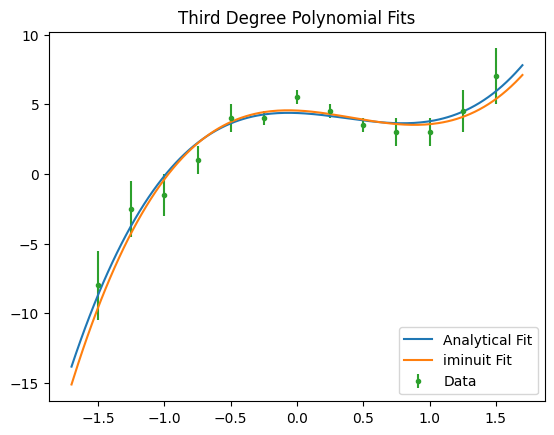
\includegraphics[width=0.4\textwidth]{Graphs/Least_Squares/3rd_deg_polynomial_fit_2}
    \caption{Comparison Between Analytically and Numerically Determined Best Fit Curves}
    \label{fig:least_squares:3rd_polynomial_analytic_and_numeric}
\end{figure}

\subsubsection{Goodness of Fit Analysis}

To analyze how well our model fits the data, we use the final minimized sum of the square residuals. For this we simply input the fit parameters which by definition minimize this value into the function \autoref{eq:least_squares:sum_square_residuals_matrix_representation}. With the given data, \( \chi_\mathrm{obs}^2 = \num{10.5} \).

To understand this value, we compare it to the family of distributions which the statistic should come from. As previously explained, it comes from the \( \chi^2 \)-distribution. Its general form was given earlier in \autoref{eq:introduction:chi_square_distribution}.

The number of degrees of freedom is the total number of data points minus the number of fit parameters: \( 13 - 4 = 9 \). Knowing this, we can plot the $\chi^2$-distribution for this number of degrees of freedom in \autoref{fig:least_squares:chi_square_distribution_1}. This lets us compare the test statistic of our fit with the expected distribution.

\begin{figure}[htbp]
    \centering
    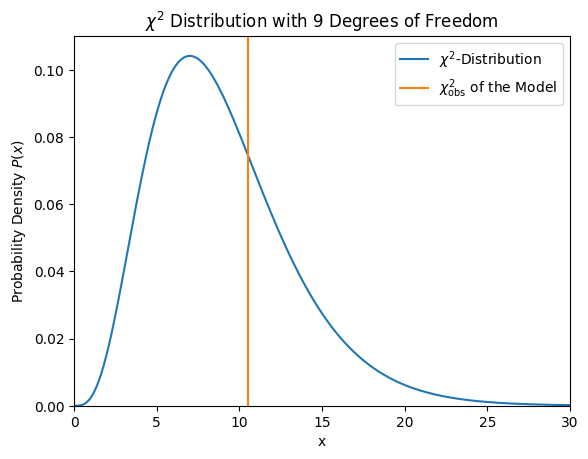
\includegraphics[width=0.4\textwidth]{Graphs/Least_Squares/chi_dist_9_dof}
    \caption{\( \chi^2 \)-Distribution with \num{9} Degrees of Freedom, Comparison to Test Statistic of the Fit Function}
    \label{fig:least_squares:chi_square_distribution_1}
\end{figure}

Using the cumulative density function of the distribution, we can calculate the \( p \)-value of the fit: \( p \approx \num{0.310} \). Its relevance will be explained in the discussion.

\subsubsection{Plotting the Best Fit Curve}

Next we want to visually plot the fit curve, using the calculated parameters. In addition to this, a \( 1 \sigma \) band should be plotted around the model curve itself. This will give a better idea about how certain the model is about its prediction.

To calculate the error band, as well as evaluating the fit function at every point, we use the known full error propagation formula with covariances from \autoref{eq:introduction:covariance_discrete_def}. In \autoref{eq:least_squares:covariance_error}, this formula is rewritten in matrix form. The matrix \( \sigma_y \) represents the uncertainty in the predicted \( y \)-output of the fit function. \( \mat{A} \) comes from the Jacobian \( \mat{J}(x) \) of the fit function, evaluated at the input point \( x \). Because the function is linear in the parameters \( \theta_i \), the Jacobian is always the same, as seen in \autoref{eq:least_squares:jacobian_of_polynomial_3rd_degree}.
\begin{gather}
    \sigma_y^2 = \mat{A} \mat{C} \mat{A}^\mathrm{T}
    \label{eq:least_squares:covariance_error} \\
    \mat{J}(x) =
    \begin{pmatrix}
        1, x, x^2, x^3
    \end{pmatrix}
    \label{eq:least_squares:jacobian_of_polynomial_3rd_degree}
\end{gather}

Implementing this in code gives the graph in \autoref{fig:least_squares:3rd_polynomial_fit_error_band}. To create this, we simply evaluate the function and the error as discussed above at many points and plot the results. Numerically, we could for example sample $x = 1$, where the model predicts $y = \num{3.78 \pm 0.48}$.

\begin{figure}[htbp]
    \centering
    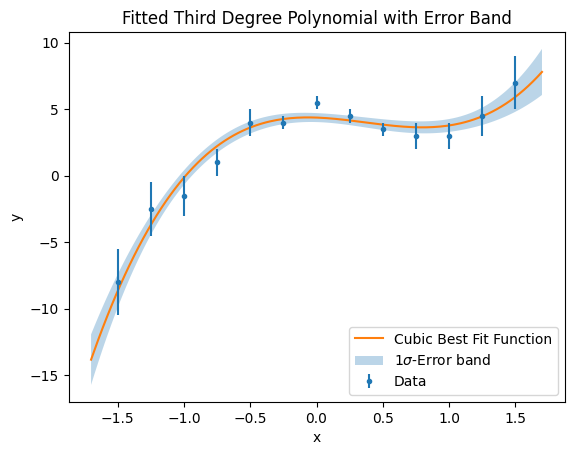
\includegraphics[width=0.4\textwidth]{Graphs/Least_Squares/3rd_deg_polynomial_fit}
    \caption{Best Fit Curve (Third Degree Polynomial) with \( 1 \sigma \)-Error Band}
    \label{fig:least_squares:3rd_polynomial_fit_error_band}
\end{figure}

\subsubsection{Fitting a Linear Model}

While the third degree polynomial seems to fit the data very well, it is of course useful to also consider other models. In this case it is not so likely, but maybe the data actually correlates linearly, in which case the more complicated model is overfitting and capturing random measurement errors.

Now we will use a linear fit function (first degree polynomial, see \autoref{eq:least_squares:linear_fit}) in much the same way as before to find a new fit with new parameters. We reuse our functions to perform the same least squares regression fit with a polynomial with only two parameters (a linear model). This time there are $2$ fewer fit parameters, meaning the degrees of freedom goes up by two: $13 - 2 = 11$ degrees of freedom.

For this fit, the parameters are given below. In \autoref{fig:least_squares:linear_fit}, we then use the same error propagation method to plot the fit function with a $1\sigma$ error band.
\begin{gather}
    y(x) = \theta_0 + \theta_1 x
    \label{eq:least_squares:linear_fit} \\
    \theta_0 = \num{3.64 \pm 0.22} \\
    \theta_1 = \num{1.5 \pm 0.4}
\end{gather}

\begin{figure}
    \centering
    \begin{subfigure}{.4\textwidth}
        \centering
        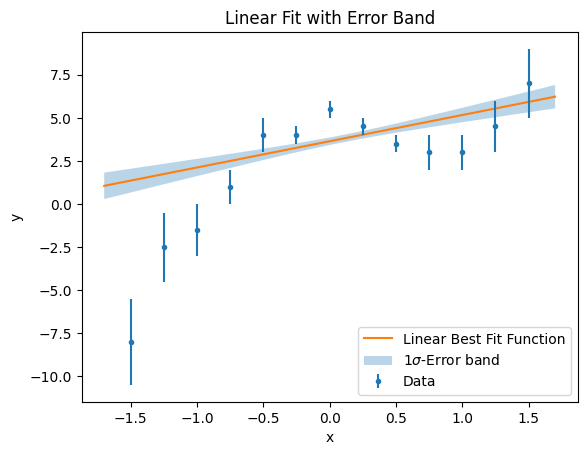
\includegraphics[width=0.9\textwidth]{Graphs/Least_Squares/linear_fit_1.png}
        \caption{Linear Best Fit Function with \qty{1}{\sigma}-Error Band.}
        \label{fig:least_squares:linear_fit}
    \end{subfigure}
    \begin{subfigure}{.4\textwidth}
        \centering
        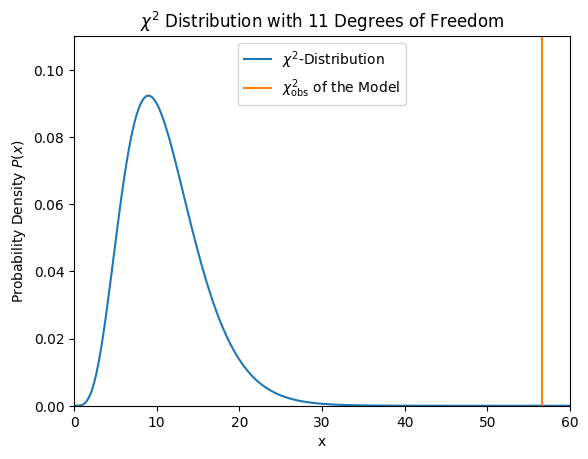
\includegraphics[width=0.9\textwidth]{Graphs/Least_Squares/linear_fit_chi_dist_11_dof}
        \caption{Corresponding \( \chi^2 \)-Distribution with \num{11} Degrees of Freedom.}
        \label{fig:least_squares:chi_square_distribution_linear_1}
    \end{subfigure}
    \caption{Best Linear Fit Function.}
\end{figure}

Lastly, we check the $\chi^2_{\mathrm{obs}}$ statistic and the $p$-value to see if the model is valid:
\begin{gather}
    \chi^2_{\mathrm{obs}} = 56.6 \\
    p = \num{3.88e-8}
\end{gather}

\subsubsection{Relationship Between Measurement Uncertainty and Resulting \( p \)-Value}

Continuing with the linear fit function, we examine what would happen if the measurement uncertainties were doubled. To calculate this we simply input the new errors into the \( \chi^2 \) function and again minimize it with respect to the \( \theta_i \).

The data with doubled error is shown alongside the best fit curve and its error band in \autoref{fig:least_squares:linear_fit_double_errors}. Uniformly changing the errors will clearly not affect the line of best fit, only the uncertainty. As we expect, the line of best fit is the same as before.

\begin{figure}
    \centering
    \begin{subfigure}{.4\textwidth}
        \centering
        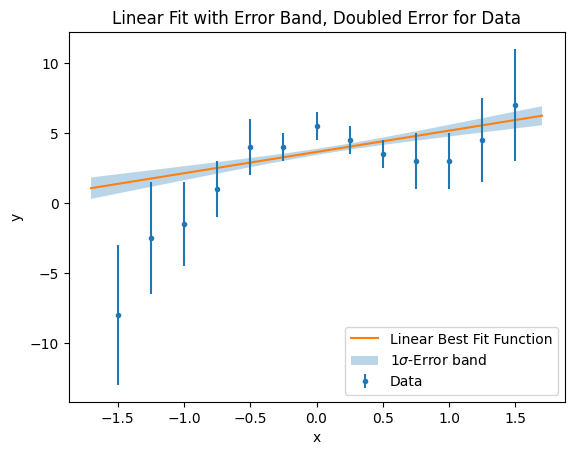
\includegraphics[width=0.9\textwidth]{Graphs/Least_Squares/linear_fit_2.png}
        \caption{Line of Best Fit and \qty{1}{\sigma}-Uncertainty Band.}
        \label{fig:least_squares:linear_fit_double_errors}
    \end{subfigure}
    \begin{subfigure}{.4\textwidth}
        \centering
        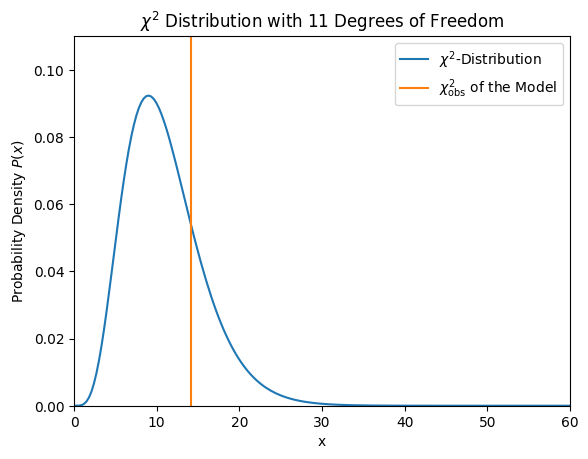
\includegraphics[width=0.9\textwidth]{Graphs/Least_Squares/linear_fit_chi_dist_11_dof_2.png}
        \caption{Corresponding \( \chi^2 \)-Distribution with \num{11} Degrees of Freedom.}
        \label{fig:least_squares:chi_square_distribution_linear_2}
    \end{subfigure}
    \caption{Linear Best Fit Function, Data with Doubled Errors.}
\end{figure}

After this, we perform the same goodness of fit analysis as before. Because the model/fit function is the same, we have the same number of parameters and the degrees of freedom remain at \num{11}. As seen in \autoref{fig:least_squares:chi_square_distribution_linear_2}, the \( \chi^2 \) test statistic is reduced a lot compared to before. This will be explained further in the discussion.

\subsection{Fitting Sample Data from Harmonic Oscillators}

Continuing with the least squares method of finding fit curves, more complicated data and models will now be examined.

In this case we are given generated data from damped and driven harmonic oscillators. One data set is measurements of displacement vs. time. Secondly we have the relationship between amplitude of the oscillation and the driving frequency.

Once again we define the two functions which we want to fit to our data sets (see \autoref{tab:least_squares:harmonic_oscillator_independent_fits}). Then we use the same method as before, defining the sum of the square residuals ($\chi^2$) as our parameter to optimize. Using \verb|iminuit| we find the parameters which minimize this function.

Similarly to before, we also do a goodness of fit analysis on the models. The most relevant value to report is the \( p \)-value for both fit functions.

Importantly, here we will apply the method completely independently to both datasets. The parameters are given below. The fit functions are plotted in the next section, see \autoref{fig:least_squares_02:position_vs_time_2} and \autoref{fig:least_squares_02:amplitude_vs_frequency_2}.

\begin{table}[ht]
    \caption{Determined parameters of the harmonic oscillators}
    \centering
    \(
    \begin{array}{rlS[table-format=+1.3(4)]|rlS[table-format=+1.3(4)]}
        \multicolumn{3}{c|}{\text{Damped Oscillator}} & \multicolumn{3}{c}{\text{Driven Oscillator}} \\
        \multicolumn{3}{c|}{x(t) = x_0 e^{- \beta t} \cos(\omega t + \varphi_0); \quad \omega = \sqrt{\omega_0^2 - \beta^2}} & \multicolumn{3}{c}{A(\omega) = \frac{K}{\sqrt{(\omega^2 - \omega_0^2)^2 + 4 \beta^2 \omega^2}}; \quad K = \frac{f}{m}} \\ \hline
        x_0       & = &  0.098 \pm 0.003 &          &   &                 \\
        \varphi_0 & = & -0.03  \pm 0.03  & K        & = & 0.199 \pm 0.005 \\
        \omega_0  & = &  4.027 \pm 0.014 & \omega_0 & = & 4.000 \pm 0.009 \\
        \beta     & = &  0.282 \pm 0.014 & \beta    & = & 0.301 \pm 0.012 \\
        p \text{-Value} & : &  0.966           & p \text{-Value} & : & 0.0458
    \end{array}
    \)
    \label{tab:least_squares:harmonic_oscillator_independent_fits}
\end{table}

% \begin{gather}
%     x(t) = x_0 e^{- \beta t} \cos(\omega t + \varphi_0); \quad \omega = \sqrt{\omega_0^2 - \beta^2}
%     \label{eq:least_squares_02:damped_oszi_fitfunction} \\
%     \begin{aligned}
%         x_0 &= \num{0.098 \pm 0.003} \\
%         \varphi_0 &= \num{-0.03 \pm 0.03} \\
%         \omega_0 &= \num{4.027 \pm 0.014} \\
%         \beta &= \num{0.282 \pm 0.014}
%     \end{aligned} \\
%     p \text{-Value}: \num{0.966} \\
%     A(\omega) = \frac{K}{\sqrt{(\omega^2 - \omega_0^2)^2 + 4 \beta^2 \omega^2}}; \quad K = \frac{f}{m}
%     \label{eq:least_squares_02:driven_oszi_fitfunction} \\
%     \begin{aligned}
%         \omega_0 &= \num{4.000 \pm 0.009} \\
%         \beta &= \num{0.301 \pm 0.012} \\
%         K &= \num{0.199 \pm 0.005}
%     \end{aligned} \\
%     p \text{-Value}: \num{0.0458} \\
% \end{gather}

%%% MOST ÜBERFLÜSSIGE GRAPHS HERE
% \begin{figure}[htbp]
%     \centering
%     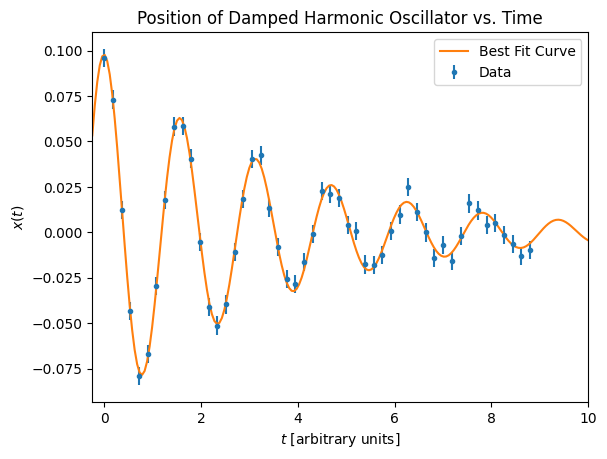
\includegraphics[width=0.5\textwidth]{Graphs/Least_Squares/position_vs_time_1.png}
%     \caption{Data and Fitted Curve for Position vs. Time of a Damped Harmonic Oscillator}
%     \label{fig:least_squares_02:position_vs_time_1}
% \end{figure}

% \begin{figure}[htbp]
%     \centering
%     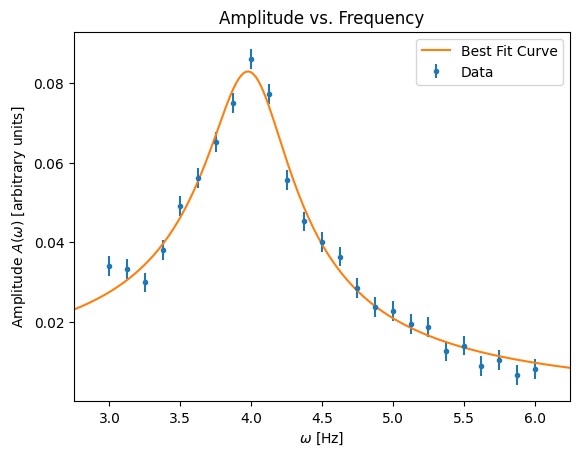
\includegraphics[width=0.5\textwidth]{Graphs/Least_Squares/amplitude_vs_frequency_1.png}
%     \caption{Data and Fitted Curve for Amplitude vs. Frequency of a Driven Harmonic Oscillator}
%     \label{fig:least_squares_02:amplitude_vs_frequency_1}
% \end{figure}

\subsubsection{Simultaneous Fit}

As discussed above, we essentially treated the analysis as if we had only made one set of measurements. But in this case, we actually have more data to inform our model. The parameters which are shared between the two fit functions should obviously be the same for both fit functions (see above for the explicit form of the functions):
\begin{gather}
    x(t ; \ x_0, \varphi_0, \omega_0, \beta) \\
    A(\omega ; \ \omega_0, \beta, K)
\end{gather}

All the data contains information about these shared parameters, so we can find better estimates of them using the combined dataset.

To take this into account, we define a new square residual function \( \chi^2 \). It is the sum of the \( \chi^2 \) functions of both models and their data individually.\footnote{If desired, during the sum the functions could be weighted to put more importance on one of the two datasets. In our case we do not do this, because both datasets are equally valid and valuable.} We obviously make sure that this function keeps the relevant parameters shared between the two functions. Minimizing \( \chi^2 \) again using \verb|iminuit| lets us find the \num{5} parameters using all the available data.

The fit parameters are given below. The new fit functions are graphed alongside the previous independently determined ones in \autoref{fig:least_squares_02:position_vs_time_2} and \autoref{fig:least_squares_02:amplitude_vs_frequency_2}.
\begin{gather}
    \begin{aligned}
        x_0 &= \num{0.0998 \pm 0.0025} \\
        \varphi_0 &= \num{0.003 \pm 0.027} \\
        \omega_0 &= \num{4.007 \pm 0.008} \\
        \beta &= \num{0.294 \pm 0.009} \\
        K &= \num{0.197 \pm 0.004}
    \end{aligned} \\
    p \text{-Value}: \num{0.543} \\
\end{gather}

\begin{figure}
    \centering
    \begin{subfigure}{.4\textwidth}
        \centering
        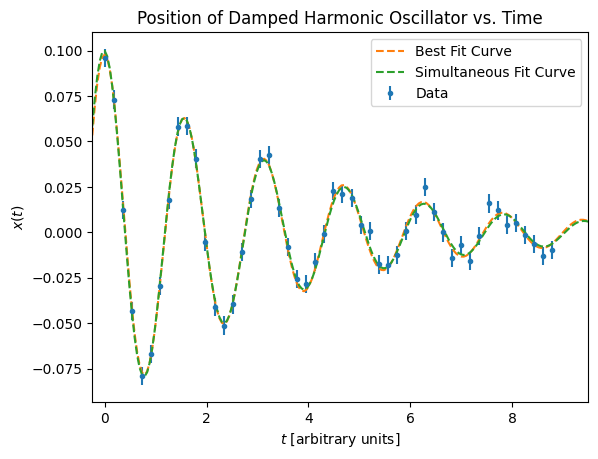
\includegraphics[width=0.9\textwidth]{Graphs/Least_Squares/position_vs_time_2.png}
        \caption{Position vs. Time}
        \label{fig:least_squares_02:position_vs_time_2}
    \end{subfigure}
    \begin{subfigure}{.4\textwidth}
        \centering
        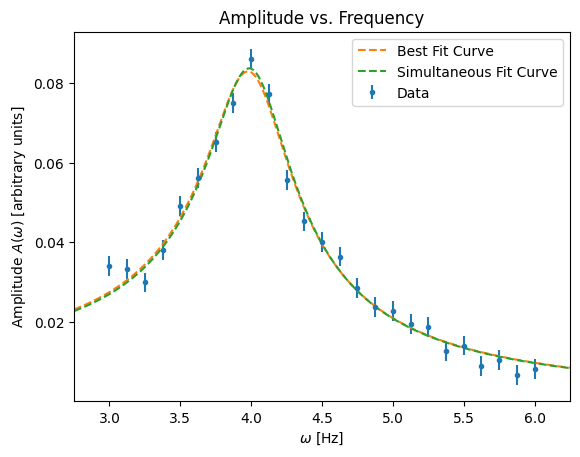
\includegraphics[width=0.9\textwidth]{Graphs/Least_Squares/amplitude_vs_frequency_2.png}
        \caption{Amplitude vs. Frequency}
        \label{fig:least_squares_02:amplitude_vs_frequency_2}
    \end{subfigure}
    \caption{Damped Harmonic Oscillator Showing Data with Independently and Jointly Calculated Fits.}
\end{figure}

We note that the \( p \)-value of this fit is quite high, giving us confidence that our combined model fits the data well.